\documentclass[sigconf,anonymous,10pt,authorversion]{acmart}
\settopmatter{printacmref=false} % Removes citation information below abstract
\renewcommand\footnotetextcopyrightpermission[1]{} % removes footnote with conference information in first column
\pagestyle{plain} % removes running headers

\usepackage{xspace} % for the spaces after the \commands,
\usepackage{yfonts} % this is for illuminated characters - can remove
\usepackage[font=itshape,noorphans]{quoting}
\bibliographystyle{unsrtnat}

\AtBeginDocument{%
  \providecommand\BibTeX{{%
    \normalfont B\kern-0.5em{\scshape i\kern-0.25em b}\kern-0.8em\TeX}}}

\setcopyright{rightsretained}
\copyrightyear{2021}
\acmYear{2021}
\acmDOI{10.1145/1122445.1122456}

% \ccsdesc[500]{Computer systems organization}

% \keywords{naming}

\acmConference[The 13th ACM Workshop on Hot Topics in Storage
and File Systems]{HotStorage '21}
%\acmBooktitle{The 13\textsuperscript{th} ACM Workshop on Hot Topics in Storage
% and File Systems, July 27-28, 2021}
\acmPrice{}
\acmISBN{978-1-4503-XXXX-X/18/06}

% Lifted the comments and choice of initials from Silos; feel free to edit as needed!
\newcommand{\nb}[2]{{\yellowbox{#1}\triangles{#2}}}
\newcommand{\nbc}[3]{
 {\colorbox{#3}{\bfseries\sffamily\scriptsize\textcolor{white}{#1}}}
 {\textcolor{#3}{\sf\small$\blacktriangleright$\textit{#2}$\blacktriangleleft$}}}
\newcommand{\version}{\emph{\scriptsize\id}}
\newcommand{\ugh}[1]{#1} % please rephrase
\newcommand{\ins}[1]{#1} % please insert
\newcommand{\del}[1]{} % please delete
\newcommand{\chg}[2]{#2} % please change
\renewcommand{\nb}[2]{\nbc{#1}{#2}{orange}}

% Margo
\definecolor{miscolor}{rgb}{0.4,0.6,0.2}
\newcommand\MIS[1]{\nbc{MIS}{#1}{miscolor}}

% Tony
\definecolor{tmcolor}{rgb}{0.5,0,0.5}
\newcommand\tm[1]{\nbc{TM}{#1}{tmcolor}}

% Sasha
\definecolor{sfcolor}{rgb}{0.2,0.0,0.5}
\newcommand\sasha[1]{\nbc{SF}{#1}{sfcolor}}

% Reto
\definecolor{retocolor}{rgb}{1.0,0.49,0.0}
\newcommand\reto[1]{\nbc{RA}{#1}{retocolor}}

% Surbhi
\definecolor{spcolor}{rgb}{0.0,0.4,1.0}
\renewcommand\sp[1]{\nbc{SP}{#1}{spcolor}}

% Joel
\definecolor{jncolor}{rgb}{0.5,0.4,1.0}
\newcommand\jkn[1]{\nbc{JN}{#1}{jncolor}}

% Ada
\definecolor{adacolor}{rgb}{1.0, 0.5, 0.5}
\newcommand\ada[1]{\nbc{AG}{#1}{adacolor}}

\settopmatter{printfolios=true} % this gives page numbering

% system name
% Kwishut is the Musqueam word for "name" (literally "to name it")
% http://www.sfu.ca/~gerdts/papers/HulquminumWords.pdf
%
\newcommand{\system}[0]{\emph{Kwishut}\xspace}

% use cases
\newcommand{\usecaseactivitycontext}[0]{\textsc{activity context}\xspace}
\newcommand{\usecasedatarelationship}[0]{\textsc{data relationships}\xspace}
\newcommand{\usecasecrosssilosearch}[0]{\textsc{cross-silo search}\xspace}
\newcommand{\usecasenotifications}[0]{\textsc{notifications}\xspace}
\newcommand{\usecasepersnamespace}[0]{\textsc{personalized namespace}\xspace}

% persons used in the use-cases (https://www.verywellfamily.com/unisex-baby-names-2759884)
\newcommand{\persa}[0]{Addison\xspace}
\newcommand{\persb}[0]{Bailey\xspace}
\newcommand{\persc}[0]{Cameron\xspace}
\newcommand{\persd}[0]{Dana\xspace}
\newcommand{\perse}[0]{Evan\xspace}
\newcommand{\persf}[0]{Quinn\xspace}
\newcommand{\persg}[0]{Reese\xspace}

% ability to explain 


% terminology
%Copy: bit-for-bit identical
\newcommand{\doccopy}[0]{copy\xspace}
%  derivation: the semantics change 
\newcommand{\docderivation}[0]{derivation\xspace}
% conversion: semantically identical but not Bit-for-Bit
\newcommand{\docconversion}[0]{conversion\xspace}


\begin{document}

\title{Position: Naming is Hard}

\author{Tony Mason}
\email{fsgeek@cs.ubc.ca}
%\orcid{1234-5678-9012}
\affiliation{%
  \institution{University of British Columbia}
  \streetaddress{201 --- 2366 Main Mall}
  \city{Vancouver}
  \state{British Columbia}
  \country{Canada}
  \postcode{V6T 1Z4}
}

\renewcommand{\shortauthors}{Mason, et al.}

\begin{abstract}
    Users store data in multiple storage silos, such as Google drive, Slack, email, Dropbox, and local file systems that mostly rely on traditional user-assigned names. A user who wants to locate a document that she saved while having a conversation with her colleague on a specific subject last month will have a hard time finding that document if she doesn’t remember in which silo it was stored or what name it was given.
    
    Prior work that introduced a \emph{Placeless} storage architecture enabled cross-silo search using semantically meaningful attributes, while other prior work used data provenance to construct a user's \emph{activity context} (e.g., what they were doing at the time they created or accessed data) to aid in document location. We take a position that despite these prior systems that demonstrated rich semantic search capabilities, we still cannot provide these capabilities using existing system APIs and abstractions. 
    
    We explain that this is not simply an HCI problem and identify the systems problems that must be solved to realize this vision. We present \system, an architectural blueprint for enabling semantically rich, multi-silo data management.
    
\end{abstract}

\maketitle

\thispagestyle{empty}


\balance

%%\yinipar{\color{blue}O}nce upon a time computer memory was \textit{ephemeral} and computer storage was \textit{persistent}--- until the day that Intel introduced \textit{persistent memory} (PMEM).  The storage community embraced pmem and declared that it was just the newest incarnation of computer storage. They built file systems that extolled the virtues of copy-on-write persistence and novel new application.  Unfortunately, they ignored the needs of applications that wanted to use it as \textit{memory}.  Fortunately, we recognized the importance of supporting applications needing to use persistent \textit{memory} for what it is --- a vastly larger amount of memory that just happens to be persistent.  The need of applications wanting large memories inspired us to build \textbf{daxFS}, the first persistent memory file system that focused on providing a secure, multi-tenant persistent memory allocator that \textit{also} optimizes the performance of persistent memory by the applications that need it.



\section{Introduction}
\label{sec:intro}

Today's file systems provide two primary functions: a way to store chunks of data and names that provide users with the familiar
metaphor of a file cabinet (i.e., folders and documents).
Much has changed since we adopted this design.
Now most data resides not on local file systems but on myriad services such as Dropbox, Google docs, Amazon S3, Microsoft OneDrive, and Github, as well as attached to communication mechanisms and applications such as email, chat, and collaborative communication platforms (e.g., Slack, Discord).
Today, just like local file systems, each of these storage solutions provides its own storage and naming mechanisms. Pity the user Alice who wants to find the file that was sent to her by Bob while they were having a slack conversation about cool papers in HotStorage 2020, if she remembers neither the name of the file nor whether she stored it in Dropbox, Google drive or her local file system.

The \emph{Placeless} architecture~\cite{placeless-tois} provided an elegant solution to this problem by enabling search across different storage silos using semantically meaningful names. Each file was annotated with a rich set of attributes, determined by the user or generated by software, and a naming service, spanning silos, searched the entire collection of user files using these semantically meaningful attributes. \emph{Placeless} was a huge improvement over isolated storage silos and semantically-poor names, but it did not solve Alice’s problem. Finding Alice's document requires that we track files across storage silos and \emph{activity contexts}. An activity context describes the other activities that were happening at the same time a document was accessed. This context might include applications, such as Slack, email or a web browser, which are not file systems in any traditional sense, but can be sources and destinations for data and for its semantically meaningful context.

The only solution of which we are aware that captures activity context is Burrito~\cite{guo2012burrito}, which used data provenance to keep track of a user’s activity context, i.e., the applications they were running and actions they were taking while examining a particular file. Unfortunately, Burrito is a desktop application that was intended neither to work across multiple devices nor to span multiple, remote storage silos. While it introduced the idea of activity context sensitive search, it did not address any of the semantic searching issues of Placeless and it did not consider the privacy consequences of storing user context in a distributed environment.

We posit that \textbf{1) user naming should be entirely decoupled from local naming and 2) users need customizable and personal namespaces.}
We present \system\footnote{\system means ``naming'' in a native North American language.}, an architecture embodying this position, leveraging existing infrastructure where possible and extending it where necessary.
\system uses separate metadata and naming services coupled with user activity monitors.
\system is designed to allow incorporation of existing storage, metadata, and naming services without modification, while providing enhanced functionality when services support \system features.
We limit discussion to the systems infrastructure required to realize this vision; current storage management interfaces (e.g., file browser) can use \system namespaces directly, while the availability of rich metadata in \system enables HCI research on better ways for users to identify and find their data.

We begin with use cases motivating the need for \system (\S\ref{sec:use-cases}), highlighting specific features missing from today's storage and naming services. Next, we present the \system architecture (\S\ref{sec:arch}) and future research directions it enables (\S\ref{sec:future}).
We then discuss how \system builds upon prior work
(\S\ref{sec:background}) and conclude summarizing our position (\S\ref{sec:conclusion}).


\section{Why we need \system}
\label{sec:use-cases}

%%%%%%%%%%%%%%%%%%%%%%%%%%%%%%%%%%%%%%%%%%%%%%%%%%%%%%%%%%%%%%%%%%%%%%%%%%%%%%%%%%%%%%%%%%%%%%%%%%%%%%%%%
\begin{table*}[!th]
    {\renewcommand{\arraystretch}{1.3} %<- modify value to suit your needs
    \begin{tabular}{p{0.11\textwidth}p{0.4\textwidth}p{0.425\textwidth}}
         \hline
        \textbf{Feature} & \textbf{Existing Technologies} & \textbf{No Solution} \\
        \hline
        \usecaseactivitycontext &
        timestamps and geo-location, image recognition, browsing history, ticketing systems, application-specific solutions like Burrito~\cite{guo2012burrito}. &
        Link related activity across apps, record  browsing history and chat conversations relevant to the creation of the data object, storing it in ways that are secure and compact.   
        \\ 
        %
        \usecasecrosssilosearch &
        Search by name, creator, content across silos, 
        app-specific searches (e.g., Spotlight) &
        Unified search across all kinds of storage, including file systems, object stores, apps and devices 
        \\ 
        %
        \usecasedatarelationship &
        De-duplication of documents, versioning of specific files, git ancestor relation &
        Explicit notion of data identity, tracking different versions across different silos as data is transformed 
        \\ 
        %
        \usecasenotifications &
        File watchers (INotify), synchronization status, manually inspecting modified time&
        Ability to subscribe to specific changes on attributes
        \\
        %
        \usecasepersnamespace &
        Hierarchy plus hard/soft links. Use of tags. &
        Creating personalized namespaces with with flexible data organization and views 
        \\
         \hline
    \end{tabular}
    }
    \caption{Use-case driven functional requirements.}
    \label{tab:usecases}
\end{table*}
%%%%%%%%%%%%%%%%%%%%%%%%%%%%%%%%%%%%%%%%%%%%%%%%%%%%%%%%%%%%%%%%%%%%%%%%%%%%%%%%%%%%%%%%%%%%%%%%%%%%%%%%%

%Each storage silo provides a specific set of features facilitating certain use-case scenarios, for example, the local disk provides offline access to data, while cloud-based solutions allow users to collaboratively work on a shared document.

We identified five categories of information that are necessary to facilitate the integration of semantically meaningful naming with user activity context.
Unfortunately, to varying degrees, these features cannot be provided by today's storage system architecture.
We introduce these categories, summarize them in table~\autoref{tab:usecases},
and then present use cases demonstrating how they facilitate data management.

\subsection{Feature Wish List}
\label{sec:features}
\noindent\textbf{Activity Context: }
As Burrito demonstrated~\cite{guo2012burrito}, the \emph{context} in which data were accessed or created is often a useful attribute on which users wish to search, e.g., ``\emph{I'm looking for the document I was editing while emailing \persa about their favorite wines}.''
To the best of our knowledge, there is no modern system that supports queries using rich context across applications. 
We might be able to use timestamps or application-specific tags or history information in queries, but it is laborious, if not impossible, to intersect data from multiple applications and/or multiple silos.

\noindent\textbf{Cross-Silo Search: }
Users share documents in myriad ways: via messaging applications, on cloud storage services, and via online applications. Users should not need to remember which mechanism was used to share a particular document and should have some easy way of organizing and searching through a collection of such distributed documents.

\noindent\textbf{Data Relationships: }
Documents can be related in arbitrary ways. This relationship information can be used to facilitate and enable better search results. So far, we have identified three specific relationships that are particularly important: 

\noindent\emph{1) copy} is a bit-for-bit identical replica of some data, in other words two items with different names store the same data.
% Deduplication functionality in storage systems frequently takes advantage of the prevalence of copies to reduce storage consumption. However, knowing that two items with different names are, in fact, the same is also valuable information for users.

\noindent \emph{2) conversion} is a reversible, repeatable transformation that changes the representation of data, without changing its semantics, e.g., converting a CSV file into JSON.

\noindent \emph{3) derivation} refers to data that has been computationally derived from another object by altering its content, e.g., adding a row to a spreadsheet.

While storage systems can recognize copies, they cannot distinguish conversions from derivations. However, from a user's perspective, these operations are quite different: a conversion can be repeated, which is not necessarily true of a derivation.
                                              
\noindent\textbf{Notifications:}
Users frequently want to be notified when documents change, and many storage services offer this functionality.
However, users might also want notification when data on which they directly or indirectly depend changes. This requires both a notification system and an awareness of the data relationship between different objects.

\noindent\textbf{Personalized Namespaces:}
Users have different preferences and mental models to organize their documents, a source of conflict in a multi-user setting. We need a way to provide each user the ability to personalize their document structure.

\subsection{Use Cases}
The following use cases illustrate how the features described above arise in common place activities.

\noindent\textbf{Data Processing:~}
\persa and \persc are preparing a report summarizing their work on a data analysis project for a customer.
\persc sends an email to \persa containing a CSV file with original data.
\persa opens this document in Excel, formats and filters it, adds additional data from a corporate storage silo,
and then returns the Excel document to \persc on Slack.
\persc is away from their desk when it arrives, so they open it on their phone, uploading it to a cloud drive.
\persc then sends the link to \persa for editing with update notifications.
Finally, \persc sends a PDF of the report to the compliance officer who promptly asks, ``Where did this data come from?''

\noindent\textit{Feature Analysis:~}
This use case highlights the need for 1) \usecasedatarelationship, as it has instances of copies, conversions and derivations, 2) \usecasecrosssilosearch, as these items are located in multiple silos and accessed by multiple devices, and 3) \usecasenotifications, as update notifications need to be distributed to designated users.

\noindent\textbf{Delete Request:~}
Some time later, the compliance officer requests that all documents containing a customer's data must be deleted. 
To help with finding all relevant customer data, \persb joins the project and examines the report and requests the original data from which it was produced. 
\persa remembers that they gave the original data to \persc shortly after collecting it, but does not remember the name, location, or even how the relevant files were transmitted. Thus, \persa has to manually search possible locations and applications, sendsing references to documents to \persb, who then starts organizing these files to methodically identify the ones that might contain the customer's data. In the process, many of the other team members' references to the documents stop working.

\noindent\textit{Analysis:~}
This use case illustrates the need for 1) \usecaseactivitycontext to capture data that has been collected while 
interacting with the customer, 2) \usecasedatarelationship to identify related documents, 3) \usecasecrosssilosearch to easily locate relevant documents across data silos, and 4) \usecasepersnamespace to 
create a individual data organization.

% \noindent\textbf{Security and Privacy:~}
% \persg, an investigative journalist who routinely receives sensitive information from third parties, is investigating the company from the prior use cases.
% \persg needs to be able store and access sensitive information, including information about the activity context of various e-mails, documents, pictures, and audio and video files.
% While \persg ensures that these data are encrypted, they need to also ensure that they can both find information and ensure that meta-data associated with those files is both usable and properly protected across silos.

% \noindent\textit{Feature Analysis:~}
% This case requires both \usecasecrosssilosearch and
% \usecaseactivitycontext to allow \persg to gather information obtained from specific meetings or at a given time/place.
% While \persg must protect their sources, they must also be able to associate evidence with those sources to make judgement calls about their validity, so we must design security and privacy policies for attributes that accomplish both.

\subsection{From Use Cases to Architecture}
Each use case and feature class suggests capabilities that are unavailable today.
In~\autoref{tab:usecases} we identify existing technology that can be brought to bear on the problem while teasing apart the precise details that are missing.
Repeatedly, we find that critical information necessary to provide a feature is unavailable, that providing such information is non-trivial, and that obtaining it creates a collection of privacy challenges.
\section{Architecture}
\label{sec:arch}

\begin{figure}[!tb]
    \centering
    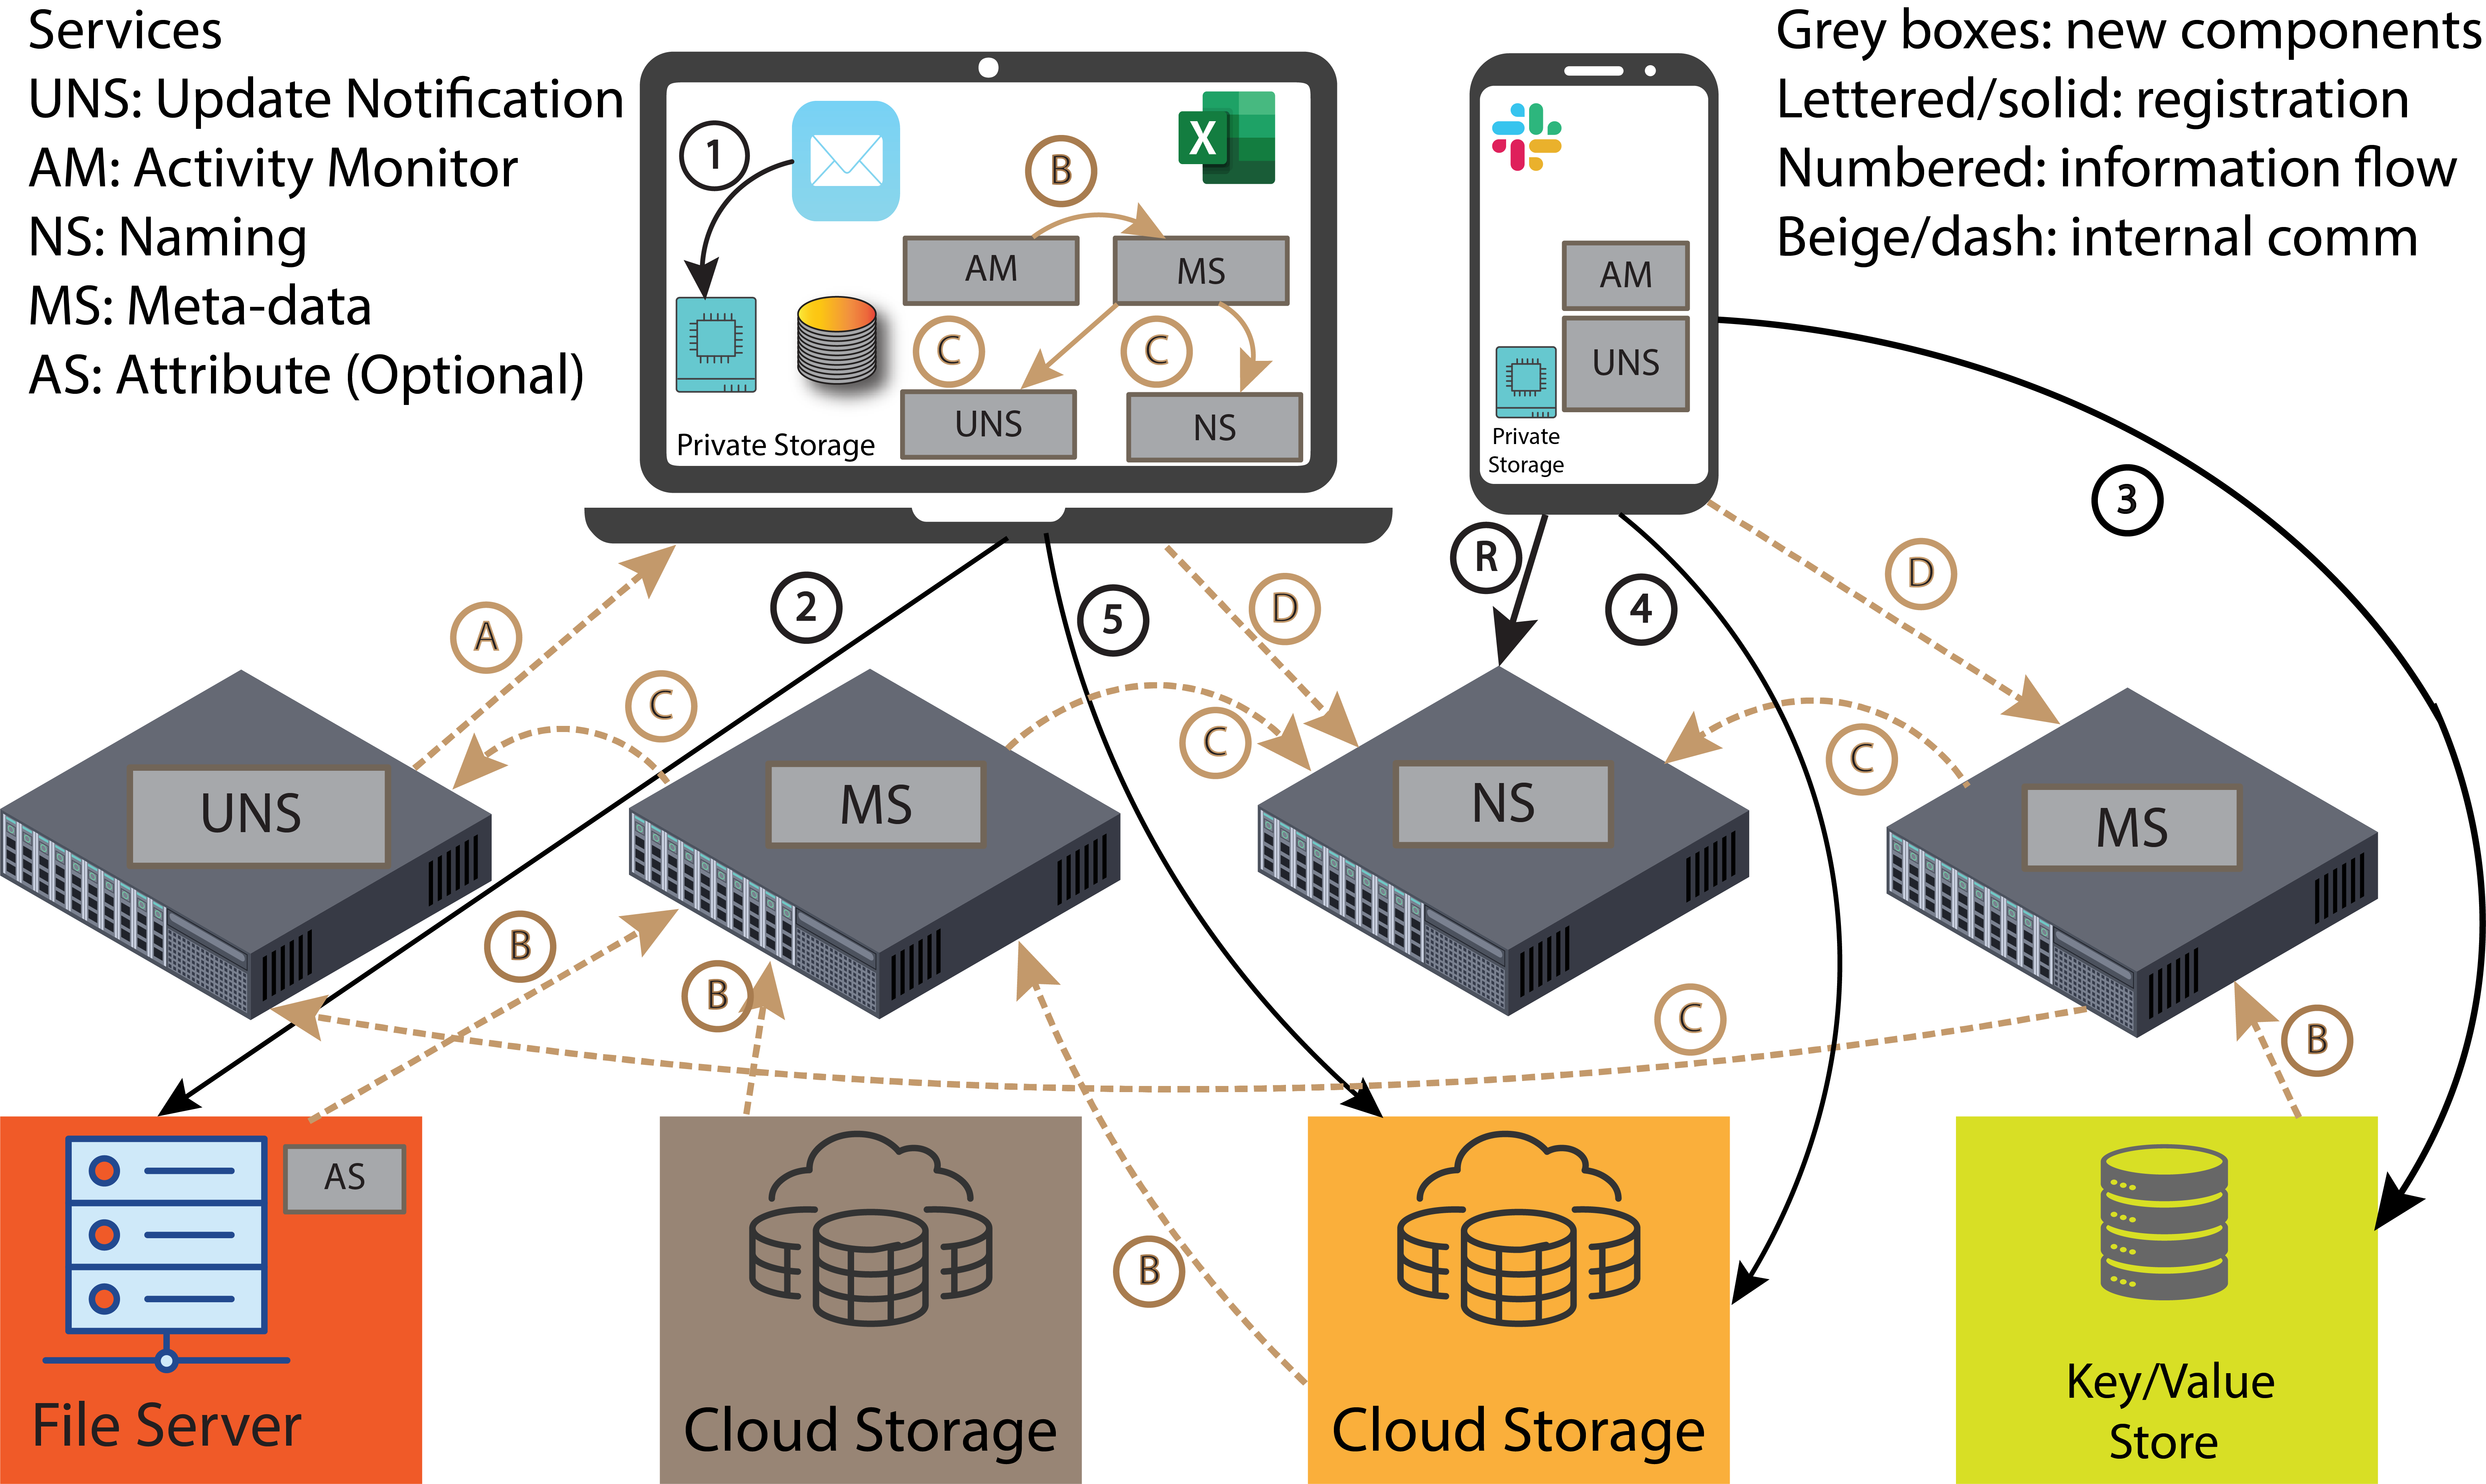
\includegraphics[width=0.45\textwidth]{figures/Naming5-legend.png}
    \caption{\system Architecture (\S \ref{sec:arch}).
    %Grey boxes indicate new components. AM=``Activity Monitor'', MS=``Meta-data Server'', UNS=``Update Notification Server'', NS=``Namespace Server''.
    }
    \label{fig:arch}
\end{figure}

%\reto{Using meta-data service that must inter-operate (federated meta data) and relationships are not first-class citizen, cannot glue the meta-data service together with naming services to enable the things we want to do. }
%\reto{the storage location is independent on the notion of related files: meta-data service treats relationships as first-class citizens. }
%\reto{get the attributes out of the silos --> currently: this is done manually}

\system is a family of services that enable sophisticated search and naming capabilities.
The key features that differentiate \system from prior work are: 
\textit{1)} incorporating object relationships as first class meta-data,
\textit{2)} federating meta-data services,
\textit{3)} recording activity context,
\textit{4)} integrating storage from multiple silos, and
\textit{5)} enabling customizable naming services.
Data continues to reside in existing and to-be-developed storage silos.
\system interacts with these silos, collects and captures metadata, and 
provides a federated network of metadata and naming services to
meet the needs of the use cases in \S \ref{sec:use-cases}.


\subsection{\system Services}

Figure \ref{fig:arch} illustrates the \system architecture. \system allows for different deployment scenarios. The five services can be run independently, they can be co-located and bundled together to run on a local device, integrated into an OS, or available as web-based services.
In the discussion below, parenthesized numbers and letters refer to the arrows in Figure \ref{fig:arch}.
There are five main components:

\noindent\textbf{1) Metadata servers (MS)}
are responsible for storing attributes and provide a superset of capabilities found in existing metadata services~\cite{federatedMetaData,smartstore}. Users can register an MS with activity monitors or attribute services, which allows the MS to receive updated attributes from storage objects and activities (B). Thus, there can be multiple sources of attributes including the user itself. Metadata servers may retain the full or partial history of attribute updates or maintain only the most recent value. 

\noindent\textbf{2) Namespace servers (NS)}
connect to one or more MS and use the metadata to provide users with a personalized namespace that allows both manual organization (i.e., a hierarchical namespace) and rich search capabilities. 
Users can register with an NS (R) that uses one or more MS to obtain relevant attributes from them (C). Additionally, users can be part of a corporate NS that allows sharing of their select metadata with other users via standard enterprise public-key cryptography.

\noindent\textbf{3) Activity monitors (AM)}
run on the user's devices. Their main function is to observe temporal relations, activity context, and relationships between objects on a user's device and transmit them to an MS (D).

\noindent\textbf{4) Attribute services (AS)}
extract attributes from storage objects and transmit them to an MS (B). An AS might be invoked on updates, run once or periodically. For example, a file system AS would update the object's metadata with basic attributes such as size or modification time. There can be many AS that extract more ``interesting'' attributes, e.g., image recognition, similarity, or other classifiers. 

\noindent\textbf{5) Update notification server (UNS)}
provides notification mechanisms. Users can register interest in changes of attributes or underlying storage and will receive a message on change events (A) to which they have access.

\subsection{\system working example}

To make the \system architecture concrete, we revisit our use-cases from \S\ref{sec:use-cases} and walk through parts of it to illustrate how \system supports the various actions and events. 

\noindent\textbf{Storing the e-mail attachment.}
\persa's act of saving the CSV file that \persc sent in email corresponds to the creation of a new object on the file server silo, i.e., the file system (4). The file server is \system-aware, so the AS co-located with it extracts attributes from the document and forwards them to the MS (B).

The AM on \persa's laptop detects that the CSV file came via company email from \persc. It then captures the activity context identifying the relationship between the e-mail and the CSV file and transmits it as additional metadata about the CSV file to the MS (that already contains metadata extracted by the AS). Moreover, because there is a company-wide namespace service, \system establishes that the e-mail attachment, the CSV in the file server, and the one on \persc's laptop (from which the file was sent) are exact copies of each other. 

Many applications already record some form of activity context, e.g., chat history, browsing history. Such histories provide a rich source of additional metadata. Other activity context, specifically the relationship between objects, such as the fact that a particular file was saved to a local storage device from an email message, requires more pervasive monitoring as found in, e.g., whole provenance capture systems~\cite{camflow}. \system is agnostic about the precise data that comprises activity context, but allows for storing and accessing activity context as metadata. 

\noindent\textbf{Creating the Excel file.}
Next, \persa opens the CSV file using Excel and stores it as a spread sheet. This creates a new object. The AM detects that the newly created spreadsheet is a conversion from the CSV file, either via a notification from \system-aware Excel or by monitoring the system calls executed on the local system. \persa proceeds to modify the data by filtering it in Excel and saving the changes. The AM records this event and updates the meta-data of the spreadsheet to record the derivation-relationship. Ideally a \system-aware version of Excel specifies to the AM the exact type of the relationship (in this case a derivation); otherwise the AM informs the MS about an unspecified data relationship by observing the opening of a CSV file and a subsequent creation of the Excel file. 

% \persa proceeds to upload the new Excel file on Slack, which triggers the creation of a new storage object as Slack creates a local copy, the addition of new metadata to MS via AS, and the addition of a \emph{copy} data relationship between the original Excel file and the Slack’s copy. The AM notices (by monitoring Slack chat) that the file was shared with user \persc and promptly notifies the MS, which adds this detail to its metadata. 

% Once \persa is done, its local MS has been updated with three new objects: the CSV file, the corresponding Excel file, and Slack’s copy of the Excel file. There is a data relationship linking all three, and the metadata informing us that the original CSV came from \persc and that the final Excel file was also shared with that same person. If \persa wanted to remember what happened to the the data from the original CSV from \persc, they could query their local personal NS, which would track down this history by querying the MS metadata.

\noindent\textbf{Sharing the spreadsheet.}
As \persc  receives the Excel file from \persa via Slack on their phone, a sequence of metadata events similar to those described earlier takes place, except the phone does not run a local NS or MS. \persc now uploads the file to the company's cloud drive (4). The MS (by way of AS) reflects the creation of a new object and records its remote location. The use of a company-wide namespace and metadata service enables \system to record that the file in the cloud drive is, in fact, a copy of the one received via Slack.  Further, \persc informs their personal NS that they wish to notify \persa about all updates to the file on the cloud drive. Thus, whenever an AS sends updated attributes to the MS, \persc receives a notification. 
% The sharing relationship between the personal NS of \persa and \persc, and the exchange of the relevant cryptographic credentials, would have been set up earlier.

\noindent\textbf{Data origin and delete requests.}
When the compliance officer asks about the origin of the data, \persc can query the corporate NS to obtain the complete history of the report. This includes the spreadsheet from which the report was derived and the e-mail or Slack messages that transmitted the files. 
The corporate NS was configured to be aware of the locations of the collaborating users' personal NS. Moreover, because of the activity contexts captured by the AM, \system is able to identify documents that were created during any activity involving the customer whose data must be deleted. Starting from these documents, and by using the relationship of documents, \persb was able to find all relevant objects and delete them, including the e-mail and Slack messages.

% \persa would have configured their personal NS to allow sharing of the metadata associated with \persc with their corporate NS, and \persc would configure their personal NS similarly. As a result, when \persc issues to the corporate NS a query asking to trace the origins of the data in the final report, the corporate NS is able to return all the history tracing back to the original CSV file.

Note that unlike existing systems, \system is able to efficiently find related objects across storage silos. Operating systems already provide users with indexing services to accelerate search of local files. This search can be made cross-silo by mounting and enabling indexing on network shares (e.g., Windows Desktop Search), or by interfacing with specific applications such as e-mail (e.g., MacOS Spotlight, or Android search). The problems with indexing on a large network storage repository are resource limitations such as bandwidth and local storage that may render the system unusable during indexing. In contrast, \system addresses these limitations by delegating indexing and storage to one or more services.
NS are responsible for providing efficient search functionality. \system uses AS to keep attributes up to date with object modifications. Lastly, \system supports coordinated search among one or more local and remote NS, allowing, for example, a user to search across both their local NS as well as their employer's NS.

% \sasha{There are a few remaining pieces that we did not mention. Please look at the commented text at the end of architecture-new.latex to see if you want to restore some of that text.}
%\subsection{The remaining pieces}

%To complete the description of \system here we fill in some of the missing details. 

%\textbf{Metadata deletion and updates.} Metadata associated with a storage object can be deleted underlying storage object is deleted or when the user is required to comply with legal requirements, such as the “right to be forgotten”. The metadata of the object is updated (via push or pull by the AS) if the object changes in the underlying storage silo or if the user (or \system-aware applications) choose to create additional metadata, e.g., run image recognition on photo files and record the names of identified places and persons.

%\textbf{Security} \sasha{I am just copying what we had in the original document, but I don't know if this is useful. Cut this? } We base our security requirements on a simple threat model that considers (1) protection of the meta-data itself and (2) protecting information that might be gleaned from activity within \system.  We assume the primary threat here is inadvertent disclosure, particularly through the use of third-party service providers. Secondary threats include the ability to verify attribute information provided by external parties, including anti-repudiation as well as tampering. \MIS{I don't understand that last sentence; do you meant that the threat is attribute spam?}

%Using public key mechanisms for signing attributes provides a standard mechanism for verifying the authenticity of the attribute itself; forged signatures can be detected using other information from the \system object.  For example, an object stored in a given silo would require use of a known set of digital signatures from the relevant authoritative name service. \MIS{That last sentence seems backwards to me; I don't understand our claims.}

%\textbf{Data relationships} While \system treats the designated data relationships automatically, users and applications can create metadata for other relationships. For example, the corporate compliance officer might find it helpful if implementations of data security policies were explicitly linked to the appropriate regulation or mandate.

\section{Future Directions}
\label{sec:future}
We now explore a few research directions that \system suggests.

\noindent\textbf{Attribute Security and Integrity.}
\system decouples naming and attributes from the storage object. This opens up a research direction on the security model of attributes themselves. Are the permissions on the attributes similar to the ones on the storage objects themselves? Can a user change an attribute in its local namespace, but not in the company wide one? This segues into the question of attribute integrity/quality: not all attribute sources have the same trust-level. For instance, a user might label an image ``dog,'' while the image recognition AS might label it ``cat''.

\noindent\textbf{Privacy.}
\system collects a lot of metadata across multiple communicating channels and storage silos, including activity data. This raises the question of how to manage these metadata in a privacy-preserving manner.

\noindent\textbf{Interface Design.}
We presented a system architecture that provides a rich context to search and organize storage objects. We envision that this will provide the foundation for new directions in HCI research: By using individual namespaces, we can dynamically organize and visualize documents and other storage objects, and seamlessly navigate and locate related documents providing a new user
experience.

\noindent\textbf{Relationship-based Queries.}
\system tracks relationships between storage objects. These relationships provide minimal data provenance~\cite{provprimer} allowin users to locate the chain of related documents originating in a specific activity context.
These relationships are most naturally expressed as graphs, where nodes are objects, and edges are the relationships between objects. Edges could have weighted-labels, indicating the type and importance of their relationship. 
This enables more sophisticated data-analysis beyond pure content-based indexing by using graph queries. 
For instance, lineage queries (i.e., tracing the history of an object) are path traversals, which are challenging to implement efficiently in conventional storage systems. This suggests that the NS and/or MS require sophisticated storage and query mechanisms.
\section{Related Work}
\label{sec:background}

\system draws on prior work in semantic file systems, using search to locate documents, and federated naming systems.

\noindent\textbf{Semantic File Systems.}
Although we introduced our desire for semantically meaningful names with reference to the Placeless architecture, the idea originated in the systems community with the semantic file system~\cite{giffordSFS}, SFS.
SFS used automatically extracted attributes to construct virtual directories that contained collections of semantically related documents.
There exist many extensions or variants on this theme such as per-process namespaces~\cite{plan9}, inverting the database/file system layering to build file systems on top of queriable databases~\cite{inversion}, 
manually tagged file systems~\cite{tagfs},
constructing semantic metadata stores from distributed storage~\cite{smartstore}, and systems that manage conventional and semantic structures in parallel~\cite{gfs}.
\system represents another step in this evolution.
It extends prior work by combining semantic naming with user activity context and is designed for today's multi-silo'd storage encompassing everything from mobile devices to desktops to object stores to cloud storage.

\noindent\textbf{Search.}
An alternative to creating a semantically meaningful name space is to enable extensive metadata-based search.
Desktop tools such as Apple’s Spotlight, Linux KDE Baloo, and Windows
Desktop Search adopt this approach.
However, breakthroughs in web search (i.e., incorporation of pagerank~\cite{page1999pagerank}) demonstrated that the relationship among objects is at least as important as the metadata itself.
The efficacy of provenance-assisted search~\cite{provsearch,uprove2,pindex} demonstrates that history, in addition to relationships enhance users' ability to locate documents.
However, searching for documents is fundamentally different from naming.
Search-based approaches rely either on a user to select the correct item from many presented or on the sufficiency of providing \emph{any} relevant document.
However, naming requires the ability to identify a specific document. \system is designed to support both searching and uniquely identifying a specific document.

\noindent\textbf{Multi-silo Data Aggregation.}
%\MIS{There is an entire market for consultants who help people manage data in multiple silos; who knew?}
%\MIS{It seems that the biologists are also really interested in multi-silo search.}
UNIX mount points~\cite{unix} are perhaps the first instance of federating namespaces.
Distributed federation, as provided by distributed file systems such as NFS~\cite{nfs} and AFS~\cite{howard1988scale} followed soon after adoption of local area networks.
With the advent of cloud storage, there has been work in federated namespaces that span 
cloud stores~\cite{scfs,federatedMetaData}. 
Nextcloud (\url{https://nextcloud.com}) allows users to connect multiple Nextcloud instances and integrate with 
FTP, CIFS, NFS and Object stores. Yet, documents are still organized in a classic
hierarchical structure. Peer-to-peer sharing networks (e.g., IPFS \cite{benet2014ipfs}) implement a distributed 
file system where nodes advertise their files to users.
MetaStorage~\cite{metastorage} implements a highly available, distributed hash table, 
% similar to Amazon's DynamoDB, %% trying to cut a line or two to get us under the limit and if we leave this here, it needs a reference
but with 
its data replicated and distributed across different cloud providers.
% MetaStore offers a key-value store interface. 
Farsite~\cite{Adya:2003:Farsite} organizes multiple machines into virtual file servers, each of which acts as the root of a distributed file system. Comet describes a cloud oriented federated metadata service~\cite{federatedMetaData}.

\endinput

\subsection{Security/Privacy}
\MIS{Do we need a fourth section on security/privacy?}\tm{I don't think so... we've hit it pretty well elsewhere}.0

Security/Privacy in cloud distributed storage: https://www.usenix.org/conference/fast14/technical-sessions/presentation/mazurek
\cite{mazurek2014toward}
\tm{I liked this reference and started looking forward from it to see if there is any more recent work.}

Fine-grain encryption for large scale storage: https://www.usenix.org/conference/fast13/technical-sessions/presentation/li\_yan
\cite{li2013horus}
\tm{I didn't see how this applied to this paper.}

Farsite~\cite{adya2002farsite} has a section on privacy and access control.

\reto{Information flow control. Maybe Nickel (OSDI)}

\cite{federatedACL}


% Possibly relevant
Intuitive navigation:
https://www.nature.com/articles/srep14719
\tm{Note this is Bergman and Whittaker, the same folks that fairly well point out humans prefer navigation over search, which is why I've tried to steer away from thinking of this as a search problem.  Whittaker is at UCSC and they have a long collaborative history.}


\section{Conclusion}
\label{sec:conclusion}

We have presented our position that we need \system, a storage architecture that decouples naming from the storage location of documents and data objects, provides customizable and personalized namespaces, and that makes relationships between documents a first class citizen. With \system, users will be able to organize, share and find their data conveniently across multiple storage silos using a rich set of attributes breaking away from the rigid, hierarchical organization.

We expect \system will enable a broad area of research in HCI exploring new ways to visualize and interact with data using the mechanism's provided by \system. Moreover, we expect \system to provide interesting scenarios for security and privacy research in storage systems.




\clearpage

%\nocite{*}

\bibliography{naming}


\clearpage
% Remove me...
%\appendix
%\section{Use Cases}

We consider the following potential use cases for our naming system:

\begin{description}

    \item[Finding historical documents] - in this common usage scenario, we are
    looking for an object that we identify by what we were doing and when we
    were doing it as well as potential subjects.

    \item[Related documents in distinct storage locations] --- in this common
    usage scenario, we are looking for \textit{related} objects that, for
    whatever reason, are stored in different ``storage silos''.  For example, we
    received a document via e-mail and then saved it on the ``Dropbox folder''
    of our local system.  The e-mail and the document are related, but we have
    no obvious way to traverse back from the document to the original e-mail.

    \item[Ability to search non-traditional storage locations] --- in this usage
    scenario, we are looking for \textit{objects} that are not stored in a
    traditional storage silo but instead reside inside some other object storage
    domain.  For example, objects in an arbitrary object store, such as the
    ubiquitous key-value store.

    \item[Cross-silo versions / Document Identity]  ---
    draft.doc that you got from your coworker via e-mail, that version you stored
    on your local drive, then the one you uploaded to Office365. Another one you've
    got from another co-worker via Slack. Nirvana will show these as different
    versions from the same logical document, possibly even the temporal relationships
    between then

    \item[Notifications] -- Allowing a user to "subscribe" to change
    notifications for critical documents; e.g., an active collaborative project
    to ensure users are notified when documents are updated (and of course
    cancel notifications when they are no longer needed/useful).

    \item[Search Results] -- What kind of searches happened during the writing
    of of another document (e.g., you are interested in the statistics of a
    search, but not particular results)

    \item[Compliance] --- Identifying related documents, including references,
    to specific material that needs to be located as part of compliance with
    legal mandates, e.g., discovery notices, GDPR data removal requests (``right
    to be forgotten'').
\end{description}


\subsection{Prior Usecase Examples}

\reto{OLD `usecases follow`}

% locating documents in general
\noindent\textbf{Locating Documents.}
Users want to search for particular documents (use-cases \\usecasehistcontext, \\usecasereldocuments).
Indexing services (e.g., Spotlight), cloud-based platforms, or tools like \texttt{grep} or \texttt{find} provide mechanisms to locate documents based on their name, date of creation or modification, or even the content of the files.
However, users often need to search different storage silos independently. This poses a burden to the user.
Worse, searching over locally mounted network attached storage (e.g., NFS or Dropbox) could mean transferring gigabytes worth of data for doing the search.
Finally, current solutions do not capture activities well such as while on a call with a customer, or while attending a webinar or conference.
Not only fail existing architecture to capture these aspects, they are also not capturing seemingly simple relationships between a file stored on disk and the e-mail exchange through which it was received and thus losing important contextual information.

% integration with non-traditional storage
\noindent\textbf{Alternative Storage.}
Traditional files are not the only way to store documents.
Today's applications may use object stores, key-value stores and data bases, or even implement their own storage container holding multiple objects (use case \\usecasealtstorage).
Moreover, applications want to protect their data from unauthorized accesses using various methods such as encryption, for example.
This makes searching hard and the user is forced to use the interface provided by the application to locate its documents, resulting in yet another manual cross-silo search.
While point solutions exist, e.g., Android search integration or export as WebDav-based file system, they are not ubiquitously available or do not allow users to search using the full range of attributes.

% document identity / cross silo version
\noindent\textbf{Document Identity.}
Documents have an identity. Writing an additional paragraph in this paper, does not change its identity. It rather creates a new version of the same document and both versions are related.
Likewise, uploading a document to cloud storage, renaming it, or converting it to a PDF also does not change its identity (use-cases \\usecasereldocuments, \\usecasedocidentity).
In contrast, taking last year's HotStorage paper as a template for this year's paper will change its identity.
While versioning is available on various storage solutions or VCS systems, it fails to capture cross-silo versions and relation ships. For example,
the document that was just received via e-mail is in fact a version of the one you have been editing yesterday, and that you have just uploaded to cloud storage for sharing with your co-worker who just sent it to you via e-mail.

% multi-device
\noindent\textbf{Multi-Device.}
Users may use various devices to access their files, each of which having different compute and connection capabilities (use-case \\usecasedevices).
For instance, a desktop machine is powerful and always connected, while a smartphone is low power and can often be disconnected. Cloud-storage or e-mail client apps on the devices provide a search interfaces that may offload the actual search to the server.
A user with two devices cannot easily look for files on the local disks and has now to do the search manually across multiple devices (similar to \\usecasereldocuments).

% attribute provenance
\noindent\textbf{Attribute Provenance.}
Traditional file systems tie the permissions to change attributes with the permissions to change the file contents.
Any user with sufficient rights can change any attribute or the file contents.
While there are systems that record the user who changed the file last, it may not capture the entire history of the changes (use-case \\usecaseattrprov).
Moreover, existing systems do not capture the intent or reason of those changes.

% attribute provenance
\noindent\textbf{Multi-View.}
A document cannot be physically present in multiple filing cabinets at the same time.
Hard and soft links provide references to other other storage locations.
However, there is still only a single physical organization of files making it impossible to organize files by year-customer, and customer-year at the same time.
File managers may offer tags, and media libraries to notion of albums and grouping by year to provide specific ways to sort, filter or organize files.
This approach, however, is not generally available and users cannot freely choose and adapt their \emph{view} of their files (use-case \\usecaseviews)

\section{Notes from the meeting (remove as pleased)}

Focus on the what the system does, with a bit of how..

\begin{itemize}
    \item Placeless + Burrito?~\footnote{\url{https://www.usenix.org/system/files/conference/tapp12/tapp12-final10.pdf}}
    \item Attributes that are not traditionally a file.
    \item GIS information is useful
    \item don't open files for extracting meta-data
\end{itemize}

Taxonomy

\begin{itemize}
 \item table what can be done what can't. 3 columns. Use-case, what can be done, what's hard.
 \item here's a structure of them. (what's easy and hard to do with today's technology) --> references to architecture section
 \item evaluation: show that we are supporting the things that are hard.
\end{itemize}

 \begin{description}
\item[Section 1] introduction
\item[Section 2] Background
\item[Section 3] Use-cases + table
\item[Section 4] Architecture
\item[Section 5] Show that use-cases are solved
 \end{description}

Different clients:

\begin{itemize}
 \item Desktop: powerful + always connected
 \item Laptop: powerful + can be offline
 \item Smartphone: low power + mostly connected
 \item Smartphone w/o data: low power + mostly disconnected
\end{itemize}

\end{document}
